\chapter{Physically interactive robogames}\label{ch:art}
\epigraph{\itshape Begin at the beginning, the King said gravely, ``and go on till you come to the end: then stop.''}{---Lewis Carroll, \textit{Alice in Wonderland}}

\section{Definition}
Since more than 10 years, video games companies operating in the mass market of entertainment have aimed at establishing a new paradigm that involve the players actively moving in front of the screen, actually interacting with the game in a three-dimensional virtual or augmented space. This often happens by constructing an immersive virtual reality game where players are plunged in an artificial world reproduced by \textit{ad-hoc} intelligent systems devices~\citep{zyda_visual_2005}. This scenario, although enabling impressive game experience often requires to wear special devices that may limit the quality of the movement possibilities~\citep{martinoia_physically_2013}.

Enabled by the increased maturity of fields like social robotics, artificial intelligence and machine learning, \cite{martinoia_physically_2013} pushes forward the idea of designing a new level of game experience: that of~\glsdesc{pirg}. They provide a definition of~\gls{pirg} adopted in this work:

``\textit{A Physically Interactive RoboGame consists of a number of autonomous agents (including software, hardware, and physical agents) of which at least one is an autonomous robot, and one is a person. These agents interact with each other in a possibly variable and unknown environment, by following some game rules, so that the human players can have fun}~\citep{martinoia_physically_2013}.''

The authors also emphasize the existence of similar attempts for presenting robots as games where, in most cases, robots act more or less as mobile pets (e.g., \cite{fujita_open_1997,shibata_emotional_1996}). In this case, interaction is often seen as limited to almost static positions, not exploiting rich movement, nor high autonomy; the credibility of these toys to really engage lively people, such as kids, cannot be high. A notable exception is Kiro~\citep{weigel_kiro-table_2005}, a robot able to successfully play table soccer even with experienced users. In the game, the movement is limited to the control of the table bars, and the game is the robotic version of a classical bar game. The interaction provided by Kiro is relatively simple, in a very structured situation, but despite of this it matches exactly the user's expectations~\citep{martinoia_physically_2013}.

Robogames can be one of the next robotic products for the mass technological market, thus demanding a large exploration of new methodologies and applications, especially for what concerns methods for enabling high autonomy, intelligence, and adaptive behavior. In this direction, a company called~\href{https://anki.com/en-us}{Anki} started to make use of artificial intelligence techniques for the task of bringing consumer robotics into physically gaming experience. During the keynote event at Apple's Worldwide Developers Conference in 2013, the company revealed its first product: Anki Drive, a racing game featuring toy-size robotic cars controlled by a mobile app that serves as an~\gls{ai} engine. In 2015, the product was considered one of the best toys available in the market, which somehow expressed the interest for this kind of real-world smart robotic game experience. 

In the game set, the cars are sensing their positions on a carpet-like track and continually exchanging data via Bluetooth with the mobile phone. The app computes possible actions and decides what each car should do based on its objective. Thus, because is the app that defines how each car behaves and creates different gameplay scenarios, the cars can have different ``personalities'' and get customized features. Despite of the app ability for orchestrating the behaviors of the cars and posit a sense of autonomous driving, players are still limited to the use of their mobile to actually drive the cars, racing against each other or taking on the~\gls{ai} (facing other cars). Players are not directly involved in physical interaction with the robot, and play a kind of \textit{indirect} \gls{pirg} through a mechanical device used as a kind of avatar representing the players themselves.

Since some years, a set of~\gls{pirg}s have been developed and tested at the Artificial Intelligence and Robotics Laboratory (Politecnico di Milano, Italy), focusing on a more direct, physical interaction with players, as defined in~\cite{martinoia_physically_2013}. As an example, the Jedi Trainer 3.0 (see figure~\ref{fig:jedi_trainer}) was developed with the goal of resembling a scene of the first Star Wars saga movie ``Episode IV - A New Hope''. The game was designed to use an autonomous drone, a Parrot quadricopter, flying around the human player (Jedi trainee) and shooting at appropriate time by making a sound recalling the shot of a laser blast. The drone always aims at shooting at the ``Jedi trainee'' (human player) chest that in turn physically interact with it using a light-saber-looking object trying to parry the drone attack. The Jedi Trainer has been successfully tested in different unstructured environments, as reported in~\cite{bonarini_timing_2014} and~\cite{martinoia_physically_2013}.

\begin{figure}[h]
  \centering  
  \framebox{\parbox{6cm}{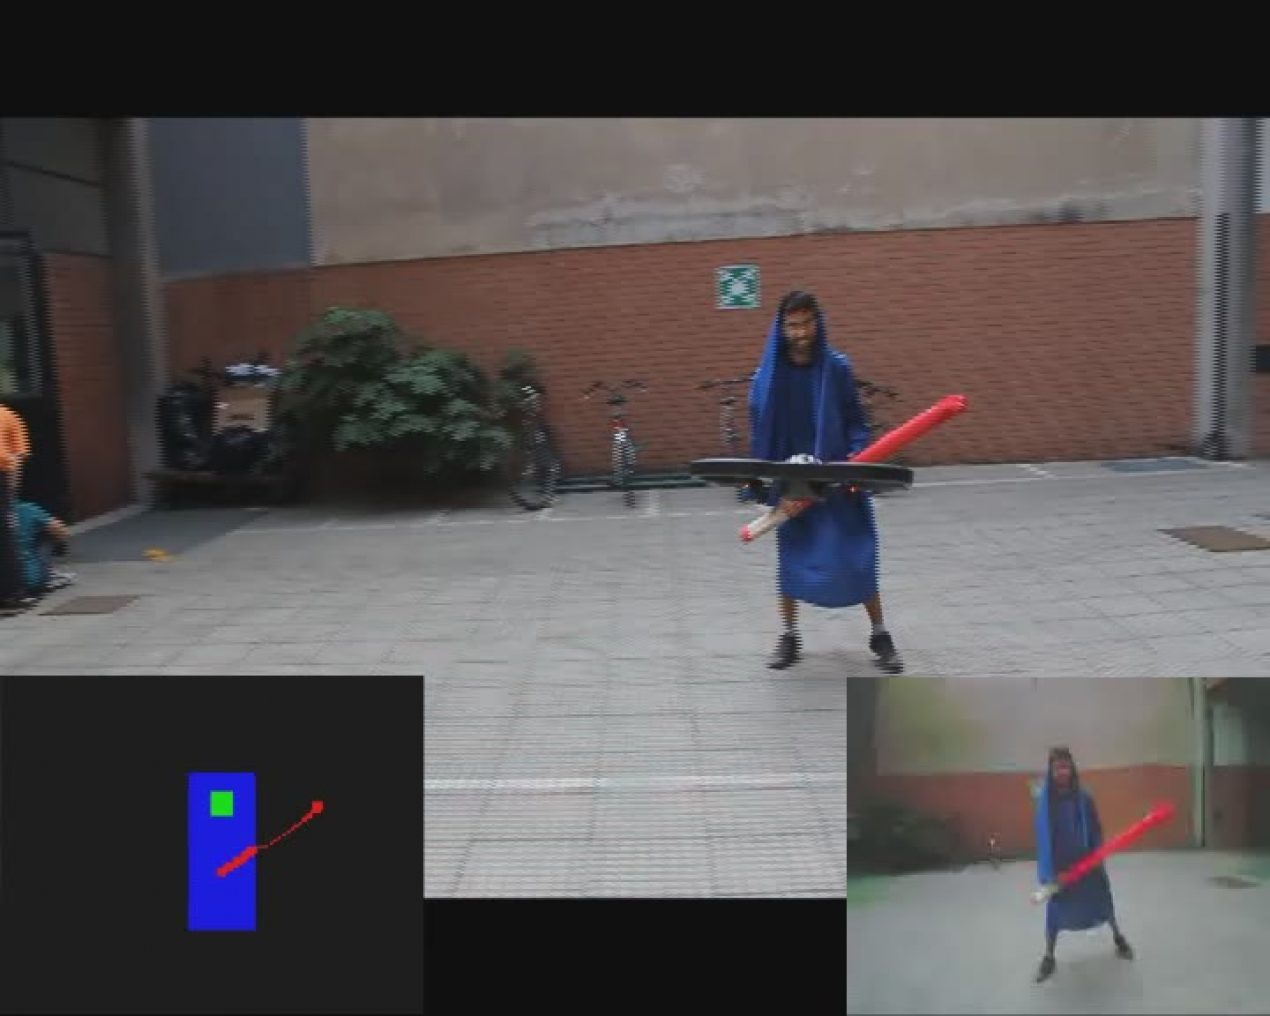
\includegraphics[ width=6cm]{images/02-art/jedi_trainer}}}
  \caption{The drone and the Jedi trainee playing JediTrainer 3.0. On the bottom right the image taken by the on board camera, on the bottom left the interpretation of the image in terms of color blobs. The green rectangle on the top of the blue one is the target where the drone is aimed at blast its laser shot~\citep{bonarini_timing_2014}.}
  \label{fig:jedi_trainer}
\end{figure}

Another example is RoboTower. It is inspired by the videogame Rock of Ages. In the game, a 30 cm high robot has to bring down a set of towers in three minutes. Human players can interact with the robot by delaying its movement through the use of cards. These cards are selected from a deck they have in their hands and put in front of the robot, which can read them when it passes over. Each card represents either an action that the robot has to execute (go back, turn around) or a deficit for its sensors (go blind), or a stop for an amount of time. A red tower correspond to the player's home and when ruined he loses; other towers are production plants that are used to recharge the delaying cards, and make them again playable after a given time proportional to the number of active plants (Fig.~\ref{fig:robo_tower}).

\begin{figure}[htp]
  \centering  
  \framebox{\parbox{4cm}{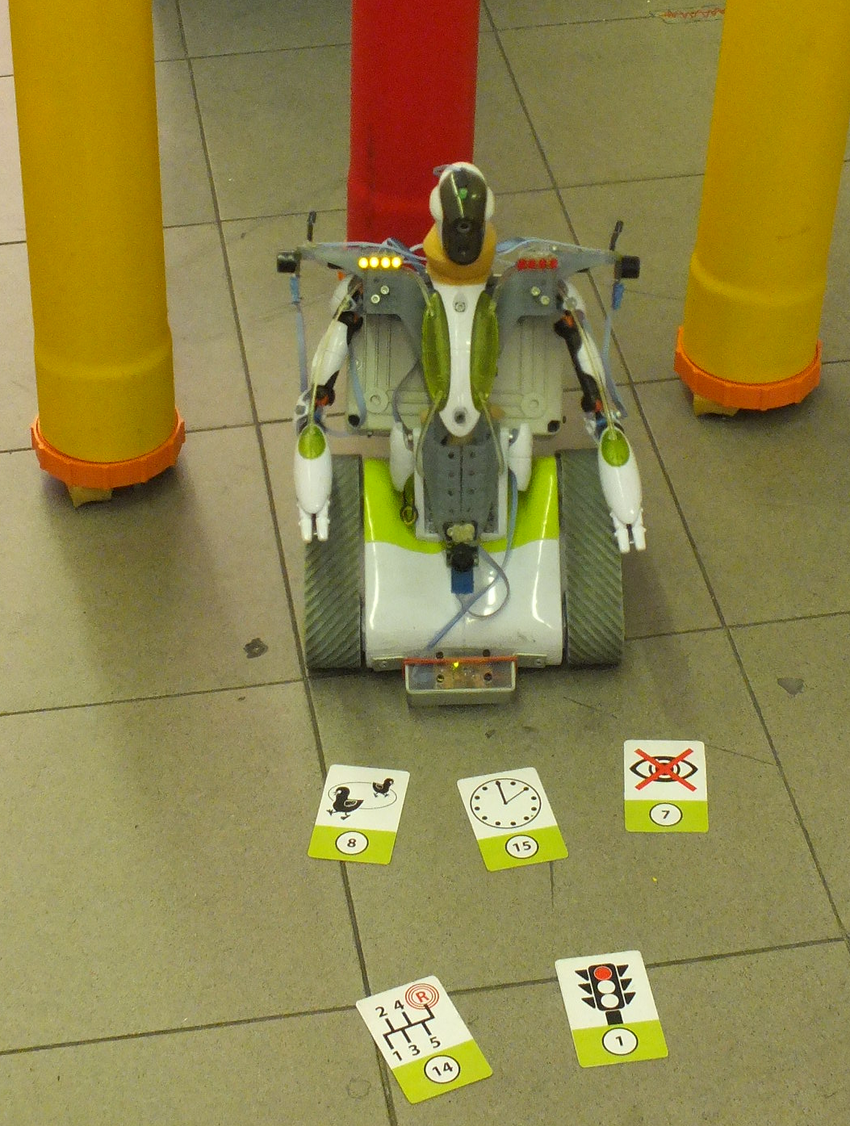
\includegraphics[width=4cm]{images/02-art/robotower}}}
  \caption{A view of the robot, the cards and the towers used in the RoboTower~\citep{bonarini_timing_2014}.}
    \label{fig:robo_tower}
\end{figure}

%ANDY Other robogames have been proposed by others in the last years and they should be at least cited, putting in evidence the absence of player's modeling.

%ANDY a taxonomy of robogames can be given here. I am developing one, and will contribute it as soon as this first reading will be finished.

As it can be easily deduced, the new application field of~\gls{pirg} and the complexity it requires prompts for a new endeavor of~\gls{hri} which is defined as the study of how humans can interact with robots, ``and how best to design and implement robot systems capable of accomplishing interactive tasks in human environments''~\citep{feil-seifer_human_2009}. Undoubtedly, robogames appears as an interesting application to investigate~\gls{hri} issues as their design process has to do not only with the technical issues of a robotic application, but it has also to consider other important aspects, including playability and usability of the game~\citep{martinoia_physically_2013} as well as user engagement and entertainment.

The necessity of investing on the research and implementation of intelligent algorithms becomes more and more evident as a way to improve~\gls{pirg} design and help to popularize the idea of having such products on the market. In particular it is important to investigate how to develop appropriate cognitive abilities in autonomous robots by the use of machine learning (ML) techniques. One example of such ability would be  intention detection for strategy adjustment. 

Also, it is important to focus on the exploration of mobile robot bases with cheap sensors and algorithms requiring little power to be executed in real time (``green algorithms") in non-structured environments, since these are constraints currently addressed in robogames, and in the whole Robotics community, in order to make robots reach a wide market. 

Properly exploiting cognitive abilities in robogames may increase the player's engagement since any apparently rational behavior of the robot may bring to accept it as a robotic companion (or opponent) ``while random actions or too complex strategies for the cognitive or perception levels of the players are perceived as not purposeful''~\citep{martinoia_physically_2013}. Due to the inherent complexity involved in the typical scenario, it is not possible to entirely rely on ``hard-coded'' abilities that are static across time and once learned by the human player tend to decrease interest. The problem of designing new interesting~\gls{pirg}s calls for the massive use of~\gls{ml}-based techniques to make sense of the obtained interaction information, thus presenting itself a new field of research.


%////////////// SEE WHETHER YOU CAN INCORPORATE SOME OF THE CITATIONS BELOW IN THE TEXT ABOVE /////////////

% Robot toys are presently the largest amount of robots delivered in our homes, at a rate of millions every year. In almost all the cases, the interaction is limited to stimulus-response reactions, but the introduction of low-cost sensors and computer power are making it possible to introduce a richer interaction and games specifically designed for mobile robots. In a~\gls{pirg}, physical autonomous (often mobile) agents are actively engaged in a game that creates some sort of interaction, either competitive or cooperative, between humans and robots, moving in the physical world. Robogames will be one of the next robotic products for the mass technological market, thus demanding a large exploration of new methodologies and applications, especially for what concerns methods for enabling high autonomy, intelligence, and adaptive behavior, in order to respond to demands in engagement support like the ones expressed in~\cite{yannakakis_entertainment_2008,yannakakis_how_2008,yannakakis_real-time_2009}. 
% Being able to evaluate how people play is crucial for an adaptive game. In the virtual game industry, several studies have been published, most of them using artificial intelligence and machine learning algorithms. For instance,~\cite{drachen_player_2009} reports about emergent self-organizing maps for grouping types of players. 

% There have been attempts for presenting robots as toys over the years, where, in most cases, the robot acts more or less like a mobile pet (e.g.,~\cite{fujita_open_1997, brooks_robots_2004}). In these cases, interaction is often seen as limited to almost static positions, not exploiting rich movement, nor high level of autonomy; the credibility of these toys to lively engage people, such as kids, are said to be constrained~\cite{martinoia_physically_2013, bonarini_timing_2014}. 

% Some~\gls{pirg}s have been reported over the last few years. Jedi Trainer 3.0.~\cite{martinoia_physically_2013} was a~\gls{pirg} mimicking a situation of the first Star Wars saga movie ``Episode IV - A New Hope'': it was able to show some apparent adaptation to the player's playing style as well as some realism of the drone's behavior, which could be understood as some kind of rational behavior by the human player.

% Queball~\cite{salter_designing_2014} was a robotic ball proposed to engage autistic children in games that could have therapeutic goals.

% Teo~\cite{bonarini_huggable_2016} is a huggable, mobile robot designed to play games with autistic children, and to provide the possibility to make free play as well as structuered play experiences.

% RoboTower~\cite{oliveira_learning_2018, oliveira_activity_2017, oliveira_modeling_2017}, where humans physically interact with an omni-directional robot by trying to protect towers while avoiding letting the robot pushing them down.
% Despite being examples of successful applications, only~\cite{oliveira_modeling_2017} and~\cite{oliveira_learning_2018} present an attempt to quantify the human behavior during gameplay.%for anonymization, while~\cite{oliveira_learning_2017} is the background work for the experiments presented in this paper.

% An approach based on genetic algorithms for capturing and modeling individual entertainment is given in~\cite{yannakakis_entertainment_2008}, where the main goal is to construct a player model, in this case a child playing a Playware game. ``Playware is the use of intelligent technology to create the kind of leisure activity we normally label play''%TODO Should this be quoted as it is from the paper?
% % [EWERTON] --> Jawohl!
% ~\cite{lund_playware_2005}. The system can predict the answers to a question asking which variants of the game are more or less ``fun''. In that work, the model is constructed from physiological signals measured during play. 

% In summary, pretty much all the related works agree that being able to label player's behavior in a game environment can enable the robotic agent to modify its interactions and playing-style in order to adapt to the skills of its human counterpart. This is a general statement shared with most human-robot interaction applications. On this work, we go further and investigate the introduction of deceptive behavior as another factor for supporting engagement.



\section{Overall design guidelines}\label{sec:dimensions}
From our experience, we have identified at least three dimension in which one must pay attention to when designing a new~\gls{pirg}. Each dimension presents its own set of utilities/challengers some of which are summarized in Figure~\ref{graph:PIRG_design_structure}. 


\begin{figure}[h]
    \centering
    \def\homomorphism{(0,0) ellipse (6.0cm and 3.5cm)}
    \def\isomorphism{(-2,0) ellipse (4.0cm and 2.5cm)}
    \def\endomorphism{(-4,0) ellipse (2.0cm and 1.5cm)}
    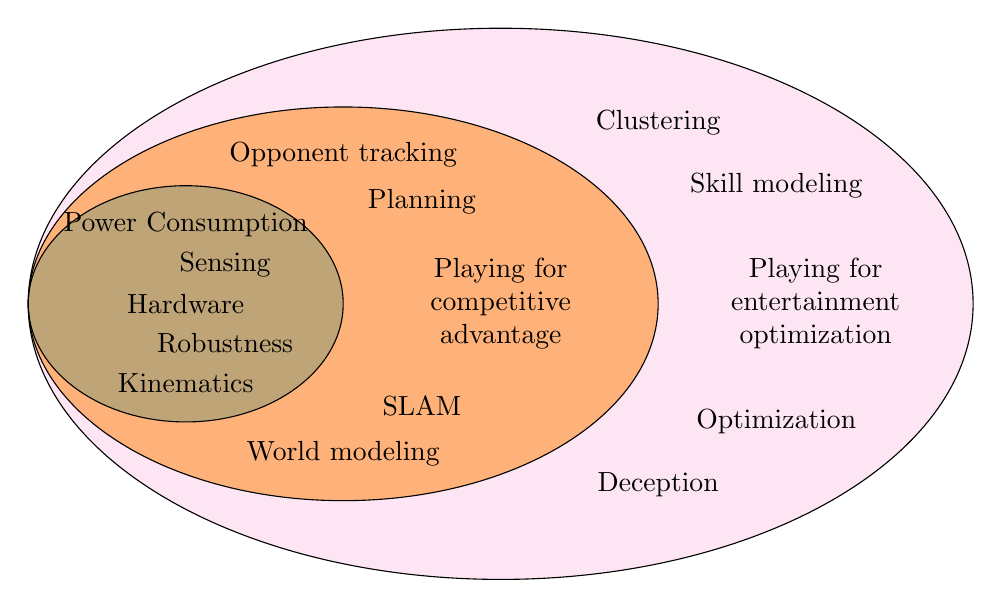
\begin{tikzpicture}
      \begin{scope}[fill opacity=0.1]
        \fill[magenta] \homomorphism;
      \end{scope}

      \begin{scope}[fill opacity=0.5]
        \fill[cyan] \endomorphism;
      \end{scope}

      \begin{scope}[fill opacity=0.5]
        \fill[orange] \isomorphism;
      \end{scope}

      \draw \homomorphism;
      \draw \isomorphism;
      \draw \endomorphism;

      {
        \scalefont{2.0}
        \node[text=black] at (-4,0) {Hardware};
      }

      {
        \scalefont{1.5}
        \node[text=black, align=center] at (0, 0) {Playing for\\competitive\\advantage};
      }
      
      {
        \scalefont{0.5}
        \node[text=black, align=center] at (-4, 1) {Power Consumption};
        \node[text=black, align=center] at (-4, -1) {Kinematics};
        \node[text=black, align=center] at (-3.5, 0.5) {Sensing};
        \node[text=black, align=center] at (-3.5, -0.5) {Robustness};
      }
      
      {
        \scalefont{0.9}
        \node[text=black, align=center] at (-1, 1.3) {Planning};
        \node[text=black, align=center] at (-2, 1.9) {Opponent tracking};
        \node[text=black, align=center] at (-1, -1.3) {SLAM};
        \node[text=black, align=center] at (-2, -1.9) {World modeling};
      }
      
      {
        \scalefont{0.9}
        \node[text=black, align=center] at (2, 2.3) {Clustering};
        \node[text=black, align=center] at (3.5, 1.5) {Skill modeling};
        \node[text=black, align=center] at (2, -2.3) {Deception};
        \node[text=black, align=center] at (3.5, -1.5) {Optimization};
      }

      {
        \scalefont{1.5}
        \node[text=black, , align=center] at (4, 0) {Playing for\\entertainment\\ optimization};
      }
    %   \node[align=left] at (  -2, 2) {Auto-\\morphismen};
    \end{tikzpicture}
    \caption{The general design dimensions for a robot in~\gls{pirg} environment. The hardware dimension is central to a~\gls{pirg} application and are the ones from which the overall robot behavior is constrained to. The playing for competitive advantage collects the systems for planning actions towards winning the game, i.e., play competitively. Playing for entertainment optimization, instead, defines the mechanisms from which the robot regulates its competitive capabilities towards making the player more engaged. This last dimension encompasses~\glsdesc{dda} approaches.}
    \label{graph:PIRG_design_structure}
\end{figure}

There are at least three basic dimensions (or problems) of interest that must be considered when building a model of this kind for \gls{pirg}s. Such dimensions are related to the specific capabilities of a mobile robot to achieve a suitable in-game performance. We delineate such dimensions as follows:

\begin{itemize}[leftmargin=*,labelsep=5.8mm]
\item {\textbf{Dimension \#1:} Fundamental robot behavior}, which concerns the fundamental aspects of the robot locomotion, timing of actions, localization and other abilities to keep it alive and well-functioning during the game play. In other words, this dimension makes up for the hardware specification of the platform. Another aspect of importance related to hardware is the case of in-game elements that are external to the robot, but important for the game interaction, \ie, those whose existence is conditioned to the game rules. An example of such elements are the cards and towers in RoboTower~\citep{bonarini_timing_2014} and towers in RoboTower v2~\citep{oliveira_activity_2017}. Despite such elements being external to the robot, one must deal with the perception of such elements and how the robot interact with them when playing.
\item {\textbf{Dimension \#2:} In-game competitive capabilities}, which are more related to the intelligent selection of actions aimed at achieving in-game goals. In other words, this dimension captures the intricacies of planning and rational behavior, using solutions developed for dimension \#1.
\item {\textbf{Dimension \#3:} Adaptive power}, which is a higher level dimension concerned with how and when during the game to adjust the robot performance to match that of the current player.
\end{itemize}

For dimension \#1, the designer should care about the setup of an appropriate robotic platform, including aspects like: electrical disturbances, power consumption, kinematic constraints, processing capabilities, sensing, robot physical structure and safety. These are recurrent aspects that must be appropriately dealt with. 
Dimension \#2 encompasses the problem of finding a plan or strategy to achieve the robot goals. This is the problem most related to the competitive behavior the robot can impose on the human player, since action selection is driven by the tendency to maximize the robot's own pay-off. After all, the robot has to give the idea that it is at best trying to beat/help its opponent(s)/companion(s).

Dimension \#3, organically based on \#1 and \#2, defines constraints on the robot behavior such that the action selection is no longer just governed by the tendency to be competitive/helpful, but is also driven by the compelling necessity to support the player interaction, in real time, as robustly as possible. Although not essential for dimension \#2, player modeling techniques are an essential mechanism for dimension \#3. Such techniques are intended to account for the player usual behavior, thus, being useful for improving platform behavior. It is in this aspect of modeling that we concentrated most of our work, as it is going to be clear from chapter~\ref{ch:modeling}.


%\subsection{Timing issues}\label{DDA}

%As discussed previously, a desired goal for~\gls{pirg} design is to have autonomous robots able to adjust behavior towards optimizing the player experience. In the direction of achieving this result, one may see some sub-tasks that are fundamental to the problem, i.e., one must \begin{inparaenum}[\itshape a\upshape)]\item deal with the maximization of the player's expectation about the agent rationale -- making believable companion/adversarial roles be effectively implemented; \item deal with timing requirements for the design of interaction -- since asynchronous actions may hugely impact engagement; \item feature selection; and \item modeling framework -- with the aim to select one of the focuses presented on section~\ref{expOptimization}\end{inparaenum}.

Additional to the general dimensions mentioned above,~\cite{bonarini_timing_2014} presented key aspects on timing issues observed during the design of several robogames, some of which related to the structure of the game:

\begin{itemize}
\item \textbf{Duration of the game}: This is a key-point since a game should reach its end in a time that guarantees to keep the players involved and to make them enjoy it. This greatly depends on the activity to be performed. In the~\gls{pirg} case, the user's physical activity, i.e the workload, is the core of the interaction and it must be taken into account when defining the game duration so that the player can come to the end with a proper fatigue requirement. The reader is invited to think about the effect on engagement when this point is not well designed.

\item \textbf{Duration of an in-game task}: In a game, a set of tasks should be achieved. Naturally, the duration of such tasks has to be bounded by the duration of the game, or a game match. So, the duration of in-game tasks can be appropriately defined in order to provide some pressure on the players such that it may be likely to engage them, rise their interest, since an appropriate level of pressure and anxiety is related to challenge. The take-away idea here is that limiting the time available for an in-game task is a key-point to make it challenging.

\item \textbf{Duration of non-interactive activities}: In some games, there are activities that must be performed by a single player and so must have the right amount of time dedicated to them, i.e, a right period of time without any interaction with others (e.g, a solution of a problem, a recovering procedure). If these activities have to be done by human players, enough time has to be left for their accomplishment, but not too much time that could make them less challenging. On the other hand, if these activities must be performed by the robot(s), the human player should somehow be involved at the same time in some other activity, or the time dedicated to them should be short enough in order to lower the likelihood of making the human player bored, but long enough to be credible w.r.t. the storyboard of the game.
\end{itemize}

Some timing aspects related to the performance of both the human players and robot were also mentioned in~\cite{bonarini_timing_2014}.

\begin{itemize}
\item \textbf{Reaction time}: The time each player needs to react to an external event can be a constraint to be considered in game design. The human player's reactions in a physical interaction can be instinctive, thus requiring few hundreds of milliseconds to be activated, or may require some cognitive activity (e.g., reasoning, recognition), whose duration may span also some seconds. In~\gls{pirg}s, since they are often designed for a lively interaction, the cognitive load is usually relatively small, and a time around one-two seconds for a cognitive response from the human player in a challenging situation is often considered as appropriate. The reaction time of the robot player mainly depends on the time to recognize a situation, which is related to the time required to elaborate signals, which in turn depends on the complexity of the data to be analyzed and on the available computational power. Since~\gls{pirg}s are targeted in principle at a mass market comparable to the one of video games, the robots should be low cost, with simple sensors, and the available computational power might be as low as the one provided by cheap processing systems, like Arduino or Raspberry PI, up to that of an external laptop, tablet or smart phone. This might be a time constraint to be considered in game design, possibly justifying the related delays in the story.

\item \textbf{Actuation time}: Also actuation time may concern both the human and the robot player. For people, they might be constrained by some devices to dedicate time to perform an action (e.g., to perform a gesture with a WIIMote device). This might be desired to put some challenge in the game, and also to reduce the power of the human player w.r.t. that of the robot, so to make the game more even. For the robot, the actuation time might be a constraint given by the selected mechanical implementation, or might even be desired to reduce the power of the robot. For instance, if a robot could run fast enough to reach a target before a human player, it might be the case to reduce its speed so that the player can compete with it with some possibility to win.
\end{itemize}

Some other timing aspects are related to the establishment of a relationship.

\begin{itemize}
\item \textbf{Opponent behavior detection time}: Playing with artificial entities is engaging if the human player forgets the status of the opponent and attribute to it some human-like abilities. In particular, human players would like to play with entities that show some intelligence and intentionality. A way to achieve this status is to understand why the entity is performing an action, and, in general, what is its behavior, and what it aimed at. This may require an amount of cognitive activity proportional to the complexity of the behavior. In the mentioned experiments turned out that a random behavior is perceived as not interesting: the player believes that it is not worth to spend time with a silly entity. A too complex behavior is perceived as a random one, mostly because in~\gls{pirg}s there is not much time to reason in a cool way on all the aspects of the perceived actions. A good behavior is one that requires a short time to be detected: not too short to consider the robot as ``too simple minded'' to play with, but also not too long to dismiss the cognitive activity of trying to understand it while the player is confronting the robot.

\item \textbf{Credibility}: Each action should have a motivation, and should be credible w.r.t. the perceived motivation. Timing of the action should be consistent with this. For instance, if the robot seems to take a decision about what to do, the consequent action should last until there is a good motivation to change it. For instance, if a autonomous robot would change its movement direction randomly, there would be no apparent reason to motivate the change, and the robot would be perceived as silly. This, of course, depends on the~\gls{pirg}. In Jedi Trainer 3.0, for example, a random decision about the direction to take is consistent with what the robot is doing: trying to find a gap in the trainee guard.

\item \textbf{Activity pace}: Each player is assumed to do actions with a purpose for the game. Since they are interacting, the activity pace should be similar: a different pace, a different time between the selection of subsequent actions, would be perceived as if one would be favored w.r.t. the other one. Uneven games, in one sense or the other, are usually not appreciated.

\item \textbf{Timing perception}: In interaction, timing is a subjective perception, and it can be modified by the interaction mood, or media, or by external devices. If there is an exchange, its pace can be modified by a ``modeling and lead'' strategy. If there is a time limit to perform a task, the perception of its urgency might be further increased by taking a faster pace in all movement changes, or also by simply giving relevance to the time-to-end, e.g., by adding rhythmic lights, sounds, or clocks.
\end{itemize}

\section{Considerations}

This chapter is aimed at the presentation of relevant aspects and popular papers in the field of player modeling both to the extent of maximizing competitive advantage (section~\ref{compadvantage}) and experience optimization (section~\ref{ch:review_playing_optimization}). Despite the fact it is not supposed to be an exhaustive review of literature (for which the reader may refer to papers mentioned in section~\ref{reviews}), it was enough to spot interesting aspects one must consider when trying to achieve similar goals on~\gls{pirg}s. The motivation for this chapter was that of providing some insights, based on related literature, that might support the design of adaptive behavior in~\gls{pirg}s. 
